\chapter{ CONCLUSIONES}
\begin{itemize}
  \item[$*$]Se detectó patrones secuenciales que permiten predecir el comportamiento de fenómenos
    climáticos y su impacto en áreas con potencial de radiación solar dentro del departamento de Nariño.

  \item[$*$]Se construyeron mapas energéticos con el componente solar en el departamento de Nariño,
  usando los sensores Landsat 7 y MODIS, además se construyeron series de tiempo para radiación solar y nubosidad.

  \item[$*$]Las imágenes sateliatles son una gran fuente de información debido a la capacidad de almacenar gran cantidad de registros históricos 
  para diferentes tipos de datos, estos datos poco a poco estan siendo utilizados por organizaciones para determinar características terrestres, 
  fenómenos naturales, condiciones de los mares, características de la vegetación, etc. Por esta razón el uso de imágenes satelitales en la investigación 
  da resultados aproximados y a bajo costo, teniendo en cuenta el costo que puede implicar hacer muestreo en campo. 

  \item[$*$]Como se observó en la validación de los datos resumida en la Tabla~\ref{tabla:validacion} hay un buen porcentaje de fiabilidad para la estimación 
  del radiación solar en las estaciones activas; mediante este hecho se puede plantear que el registro histórico construido para todo el departamento de Nariño, 
  permite tener gran certeza para la toma de desiciones al momento de instalar plantas a base de energía solar en una zona determinada; un resultado agregado al 
  estudio es la identificación de la presencia de nubosidad la cual es fundamental para una óptima generación de energía a base de paneles solares o energía 
  térmica, adicionalmente se puede utilizar los datos de radiación para contemplar los efecto en el tiempo que presenta el sol sobre la vegetación. 

  \item[$*$]La detección de patrones en la serie de tiempo pemite establecer un periodo de tiempo para un óptimo aprovechamiento de las plantas solares 
  debido a que se garantiza un número determinado de dias en los cuales se presentará altas tasas de radiación solar y baja probabilidad de nubes. La metodología 
  para la detección de patrones yá se encuentra establecida para poder ser aplicada a todo el departamento.

  \item[$*$]Las herramientas de software libre son adaptable a las necesidades de los usuarios y productos como LandSat y MODIS de libre descarga presenta estanadres 
  de calidad para los cualquier tipo de estudio.

  \item[$*$]Se realizó una mejora a las estimaciones de radiación presentes en la actualidad, debido a que el reporte generado por el IDEAM no permite observar la 
  diferencia ni cambios de radiacíon sobre el territorio nariñense Figura~\ref{fig:ideamvsmodis}.
  \begin{figure}[htb]
    \centering\subfigure[Información de radiación solar presentada por el IDEAM para el departamento de Nariño]{\label{b1} 
    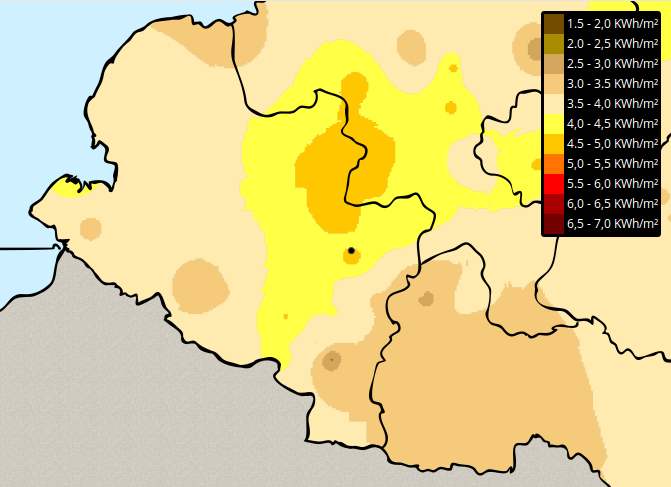
\includegraphics[scale=0.3]{pictures/narinoideam.png}}
    \centering\subfigure[Información de radiación solar producto de la investigación para el departamento de Nariño]{\label{b2} 
    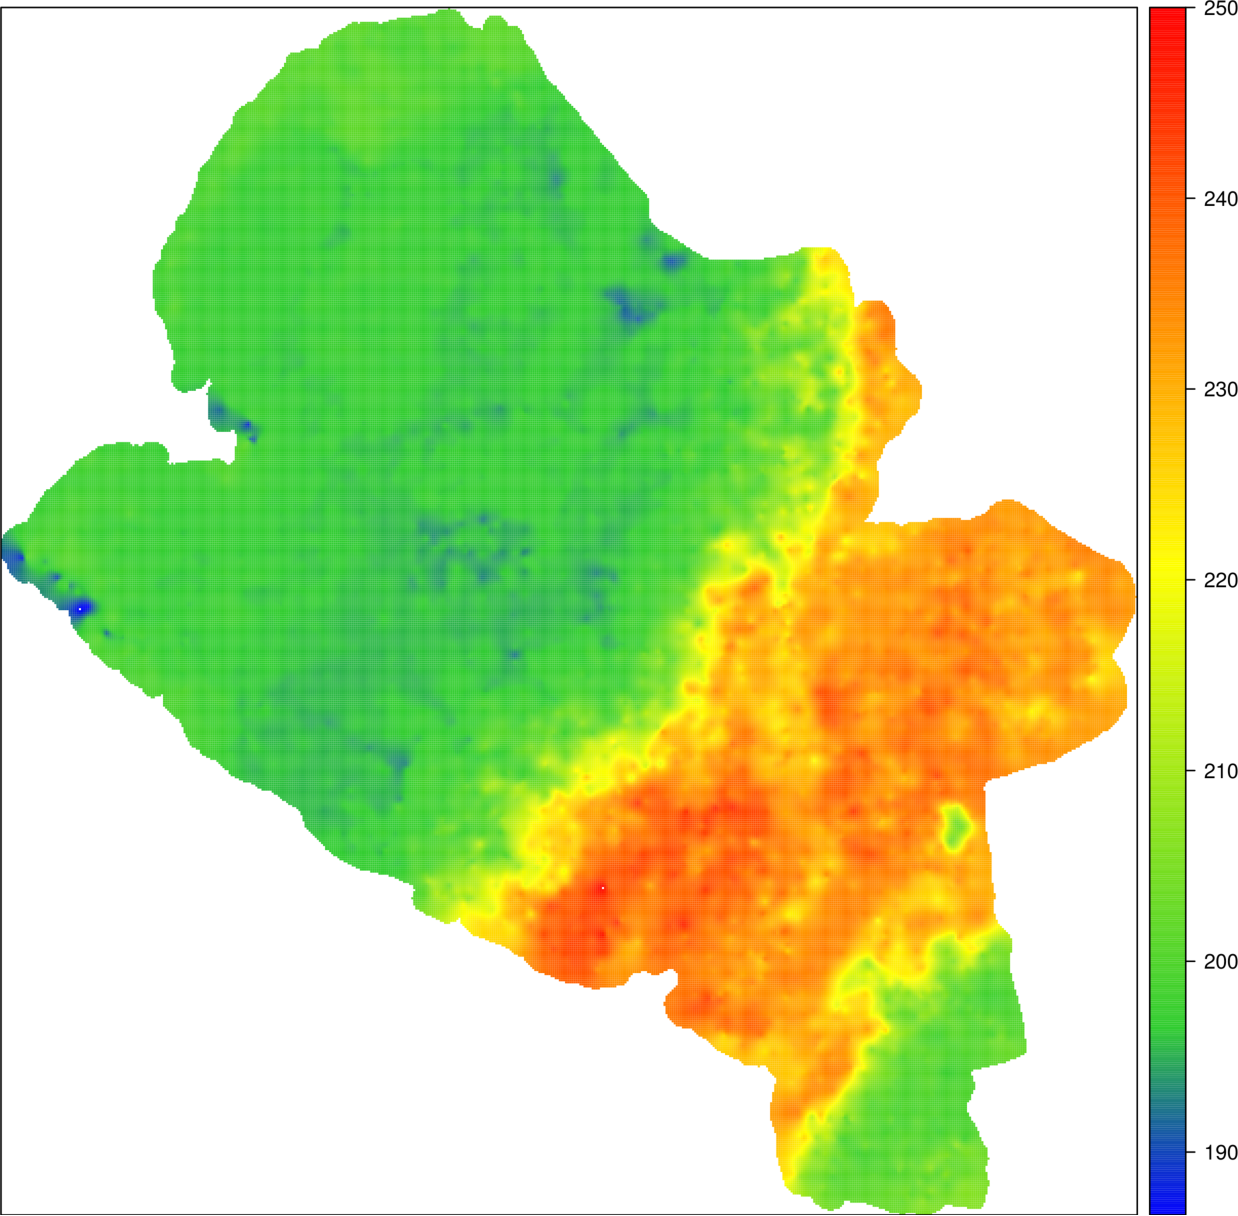
\includegraphics[scale=0.35]{pictures/general.pdf}}
    \label{fig:ideamvsmodis}
  \end{figure}

  \item[$*$]Se construyó una metodología para la construcción de mapas energéticos con el potencial de radiación solar, el cual se lo puede aplicar en zonas 
  pantropicas de Colombia utilizando imágenes satelitales de los sensores Landsat o MODIS.

  \item[$*$]Además se obtuvieron los siguientes productos:
  \begin{itemize}
    \item 11 mapas solares por año con el sensor MODIS.
    \item 12 mapas solares por mes con imágenes satelitales del sensor MODIS. 
    \item 16 mapas solares por año con el sensor LandSat.
    \item 12 mapas solares por mes con imágenes satelitales del sensor LandSat. 
    \item Serie de tiempo de radiación solar diaria para el departamento de Nariño.
    \item Serie de tiempo nubosidad diaria presente en el departamento de Nariño.
    \item Algoritmo para detección de patrones secuenciales solares.
    \item Algoritmo de detección de patrones secuenciales para nubosidad.
    \item ``GEOAlternar`` Plataforma para la visualización del potencial energético dentro del departamento de Nariño.
    \item Articulo para revista, el cual esta en proceso de evaluacion denominado: Análisis de regresión para el calculo de irradiación solar en el 
    departamento de Nariño (Colombia) utilizando imágenes satelitales Landsat y MODIS.
  \end{itemize}
\end{itemize}

\chapter{TRABAJOS FUTUROS}

La construcción de la serie de tiempo puede ser replicada para todo el territorio colombiano, debido a que se planteó una metodología y actualmente no se cuenta con una
fuente que permita ver a detalle estos tipo de variables climaticas. En la Figura~\ref{fig:colombia} se puede observar el producto MOD09GA y la dimensión con respecto al 
territorio de nariño, con esta observacion se puede concluir que hay facilidad para replicar la metodología hacia los 31 departamentos que componen a Colombia.
\begin{figure}[htb]
  \centering
  \subfigure[Tamaño de la imagen satelital respecto al departamento de Nariño]{\label{b1} 
  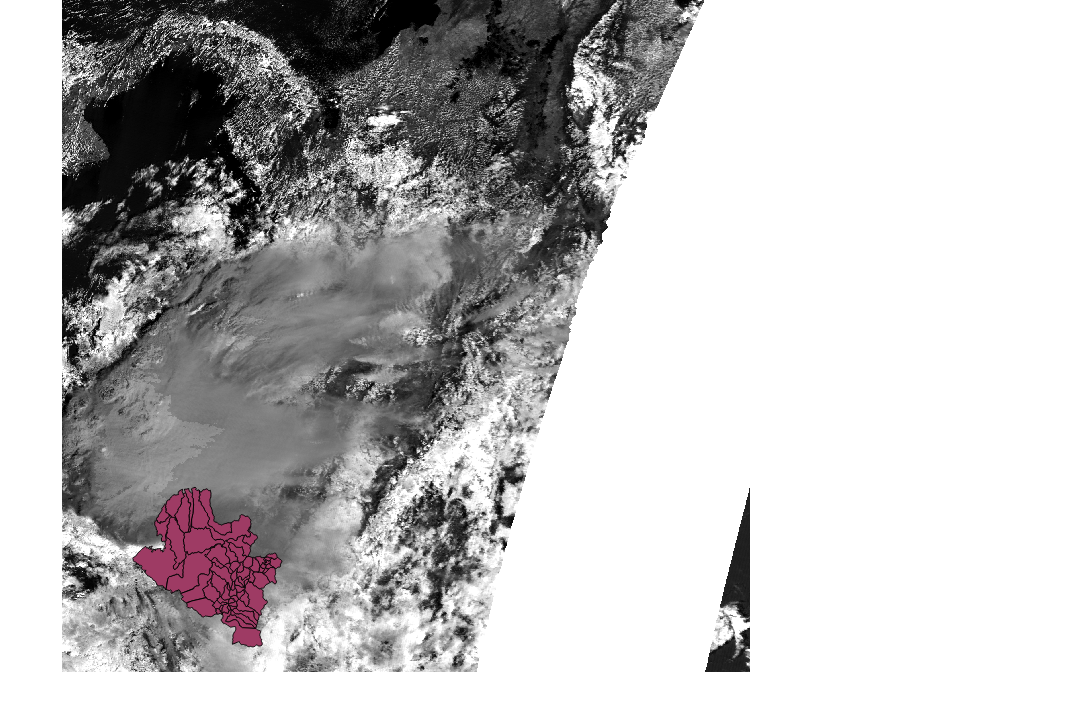
\includegraphics[scale=0.3]{pictures/ncm.png}}
  \subfigure[Dimension de territorio colombiano]{\label{b2} 
  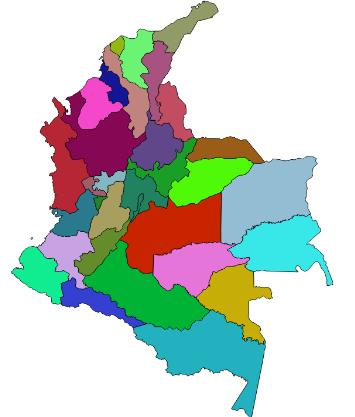
\includegraphics[scale=0.35]{pictures/colombia.png}}
  \label{fig:colombia}
\end{figure}

Las imágenes satelitales permiten versatilidad de estudios debido a las propiedades de los sensores con los que cunenta cada satelite, por estas características se puede
enfocar estudios en:

\begin{itemize}
 \item Comportamiento y tipos de vegetación en una región.
 \item Temperatura sobre una región.
 \item Presipitaciones de un territorio.
 \item Estudios de aerosoles sobre una región.
 \item Incendios y efectos sobre las regiones.
 \item Comportamiento de los mares en el tiempo.
 \item Identificación de Biomasa.
 \item Determinar propiedades de la cuencas hídrica.
\end{itemize}


